\subsection{The Greedy Algorithm}
\label{greedy}
The results in the previous section concentrated on producing nearly
optimal solutions in expectation. In this section, we will show that
it is possible to obtain good solutions regardless of the model that
generated the recommendation subgraph. \vs

We analyze the following natural greedy algorithm
that builds a $(c,a)$-recommendation subgraph iteratively as follows. 
Consider each vertex in $R$ that has not been selected
into $H$ in some arbitrary order. If there is some $v \in R$ that has $a$ neighbors
in $L$ all of which have degree less than $c$, add $v$ and these edges to $H$ breaking
ties arbitrarily.

\begin{thm}
The greedy algorithm achieves $1/(a+1)$-approximation ratio for the $(c,a)$-graph
recommendation problem.
\end{thm}
\begin{proof}
Let $R_{GREEDY}, R_{OPT}\subseteq R$ be the set of vertices that have
degree $\geq a$ in the greedy and optimal solutions respectively. Note
that any $v \in R_{OPT}$ along with neighbors $\{u_1,\ldots u_a\}$
forms a set of candidate edges that can be used by the greedy
algorithm. So we can consider $R_{OPT}$ as a candidate pool for
$R_{GREEDY}$. Each selection that the greedy algorithm makes might result in
some of the candidates becoming infeasible. But as long as the candidate pool
is not depleted, the greedy algorithm can continue. 
Each time the greedy algorithm selects some vertex $v\in
R$ with edges to $\{u_1,\ldots, u_a\}$, we remove $v$ from the candidate pool. 
If any $u_i$ had degree $c$ in the optimal solution, we would also need to
remove an arbitrary vertex $v_i\in R$ adjacent to $u_i$ from the optimal
solution. In other words, by using an edge of $u_i$, we force it to
not use an edge it used to some other $v_i$, which might cause the
degree of $v_i$ to go below $a$. Therefore, at each step of
the greedy algorithm, we have to remove at most $a+1$ vertices from
the candidate pool. Since our candidate pool has size $OPT$, the
greedy algorithm can not stop before it has added $OPT/(a+1)$
vertices to the solution.
\end{proof}

\begin{figure}[t]
\centering
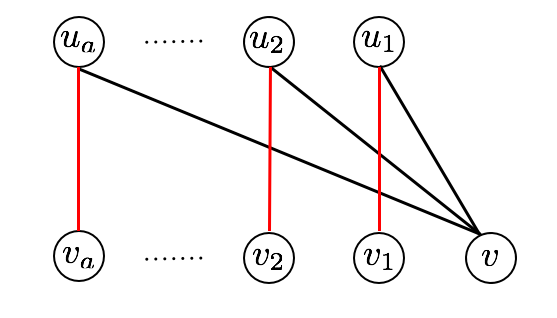
\includegraphics[width=.4\textwidth]{images/greedy.png}
\begin{minipage}[h]{.8\linewidth}
\caption{This diagram shows one step of the greedy algorithm. When $v$ selects edges to $u_1,\ldots, u_a$, it potentially removes $v_1,\ldots, v_a$ from the pool of candidates that are avaiable. The potentially invalidated edges are shown in red.}
\end{minipage}
\end{figure}

Note that this approximation guarantee is as good as we can expect.
If we set $a=1$ then we obtain the familiar
$1/2$-approximation of the greedy algorithm for matchings. 
As in matchings, randomizing the order in
which the vertices are processed still leaves a constant factor gap
in the size of the solution\cite{KarpVaziraniVazirani1990}.
Despite this result, the greedy algorithm fares much better when we
give it the same expectation treatment we have given the sampling
algorithm. Switching to the Erd\"{o}s-Renyi model instead of the 
fixed degree model used in the previous section, we now prove the
near optimality of the greedy algorithm for the $(c, a)$-recommendation
subgraph problem.

\begin{thm}
Let $G=(L,R,E)$ be a graph drawn from the $G_{l,r,p}$. If $S$ is the size of the $(c,a)$-recommendation subgraph produced by the greedy algorithm, then:
\[ \E[S] \geq r - \frac{a(lp)^{a-1}}{p}\]
\end{thm}
\begin{proof}
Note that if edges are generated uniformly, we can consider the
graph as being revealed to us one vertex at a time as the greedy
algorithm runs. In particular, consider the event $X_i$ that the
greedy algorithm matches the $(i+1)^{th}$ vertex it inspects. While,
$X_{i+1}$ is dependent on $X_1,\ldots, X_i$, the worst condition for
$X_{i+1}$ is when all the previous $i$ vertices were from the same
vertices in $L$, which are now not available for matching the
$(i+1)^{th}$ vertex. The maximum number of such invalidated vertices
is at most $\lceil i/c \rceil$. Therefore, the probability that fewer
than $a$ of the at least $l-\lceil i/c \rceil $ available 
vertices have an edge to this vertex is at most $\Pr[Y\sim Bin(l-\frac{i}{c},p): Y < a]$.
We can bound this probability by bounding each term in the binomial
expansion of it by $(1-p)^{l-\frac{ia}{c}-a+1}(lp)^{a-1}$ and obtain:

\[ \Pr[Y\sim Bin(l-\frac{ia}{c},p): Y < a] \leq a(1-p)^{l-\frac{ia}{c}-a+1}(lp)^{a-1}\]

Summing over all the $X_i$ using the linearity of expectation and this upper bound,
we obtain
\begin{align*}
      \E[S]
&\geq r - \sum_{i=0}^{r-1} \E[\lnot X_i] \geq r - \sum_{i=0}^{r-1} \Pr[Y \sim Bin(l-\frac{ia}{c},p): Y < a] \\
&\geq r - \sum_{i=0}^{r-1}a(1-p)^{l-\frac{ia}{c}-a+1}[lp-\frac{iap}{c}]^{a-1} \\
&\geq r - a(lp)^{r-1}\sum_{i=0}^{r-1}(1-p)^{l-\frac{ia}{c}-a+1} \geq r - \frac{a(lp)^{a-1}}{p}
\end{align*}
\end{proof} 

Note that at least asymptotically, this result can explain why the greedy
algorithm does much better in expectation than $1/(a+1)$ guarantee we 
can prove in the worst case. In particular, for a fixed $a$ and $c$, if
$l/r$ is taken to be a constant then this result shows that $p$ only
needs to be taken $\Theta(\log^{a}(l))$ for the greedy algorithm to
give $o(r)$ error in expectation. 
